\documentclass{article}
\usepackage{ctex}

% Set page size and margins
% Replace `letterpaper' with `a4paper' for UK/EU standard size
\usepackage[letterpaper,top=2cm,bottom=2cm,left=2.5cm,right=2.5cm,marginparwidth=1.75cm]{geometry}

% Useful packages
\usepackage{amsmath}
\usepackage{graphicx}
\usepackage{float}
\usepackage[colorlinks=true, allcolors=blue]{hyperref}

\title{微分方程数值解计算实习课后作业10}
\author{陈文宇}
\date{\today}

\begin{document}

\maketitle
\tableofcontents
\newpage
%-------------------------------------------------------------------
\section{实验结果}
%-------------------------------------------------------------------
\subsection{向后差分}

\begin{figure}[H]
\centering
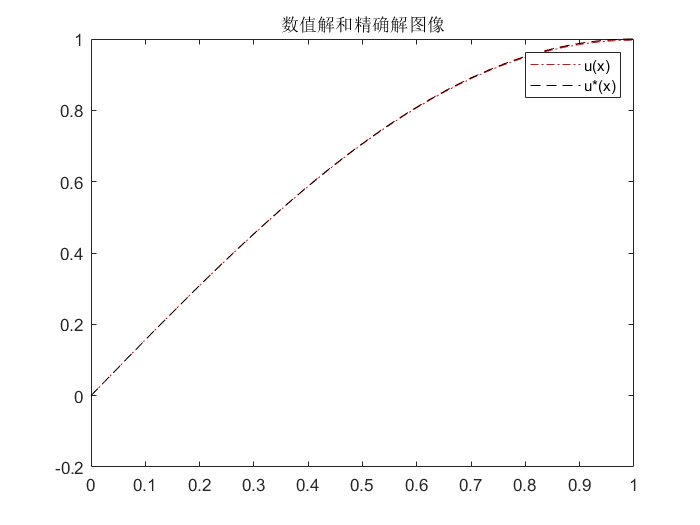
\includegraphics[scale=0.45]{向后差分/solution_1.png}
\caption{\label{solution_image}数值解和精确解的图像}
\end{figure}

\begin{figure}[H]
\subfigure{
\begin{minipage}[t]{0.3\linewidth}
\centering
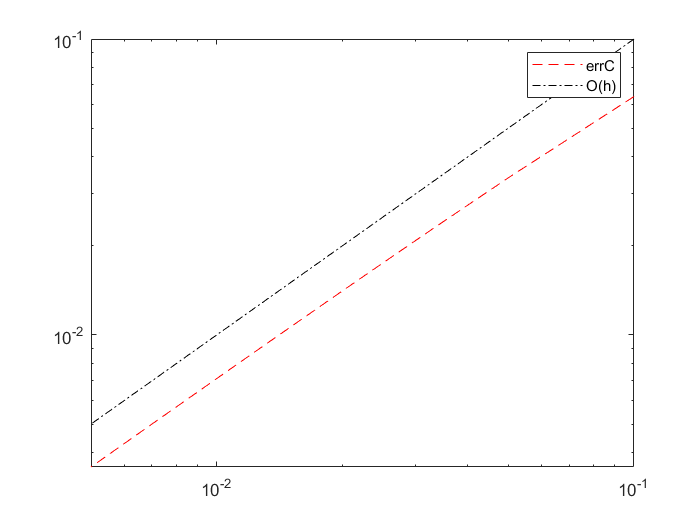
\includegraphics[scale=0.3]{向后差分/errC.png}
\end{minipage}
}
\subfigure]{
\begin{minipage}[t]{0.3\linewidth}
\centering
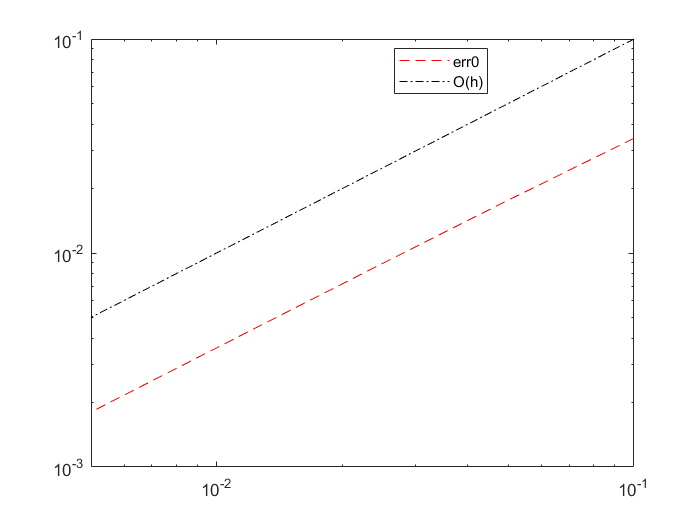
\includegraphics[scale=0.3]{向后差分/err0.png}
\end{minipage}
}
\subfigure{
\begin{minipage}[t]{0.3\linewidth}
\centering
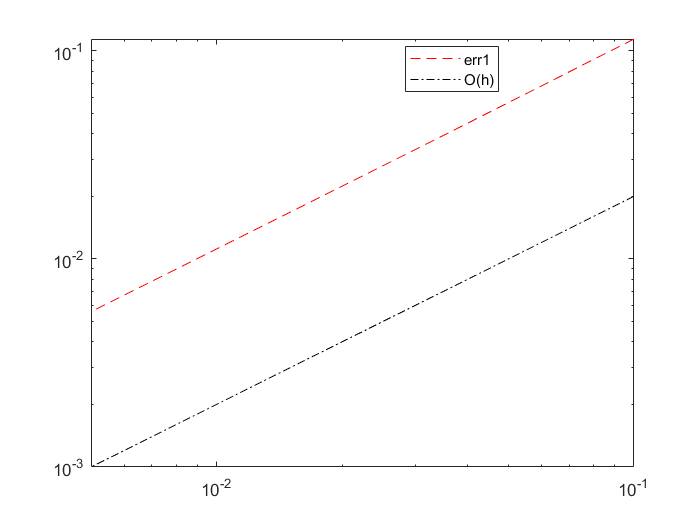
\includegraphics[scale=0.3]{向后差分/err1.png}
\end{minipage}
}
\caption{\label{solution_image}误差估计图像}
\end{figure}

\begin{figure}[H]
\centering
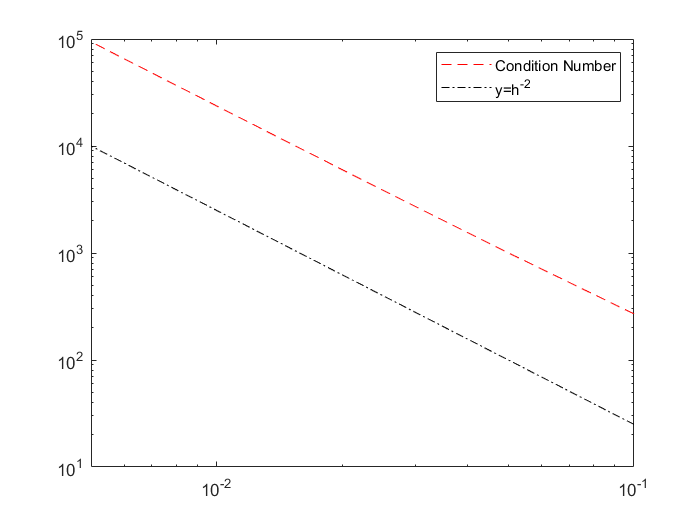
\includegraphics[scale=0.45]{向后差分/CondA.png}
\caption{\label{CondA}$CondA$}
\end{figure}

\newpage
%-------------------------------------------------------------------
\subsection{中心差分}

\begin{figure}[H]
\centering
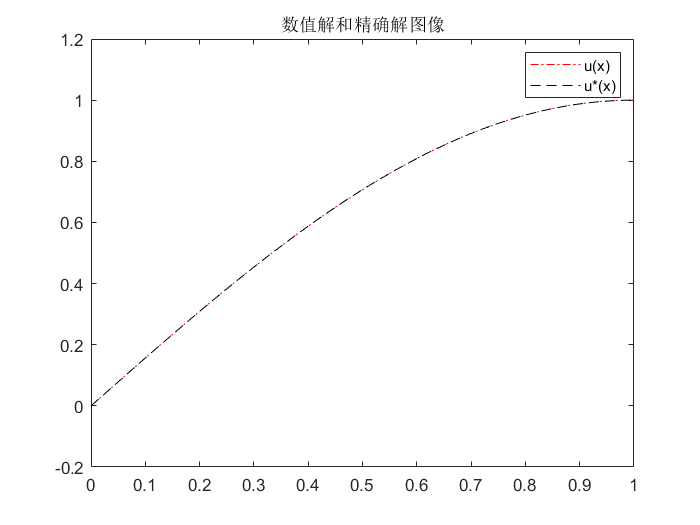
\includegraphics[scale=0.5]{中心差分和有限体积法的中矩形公式/solution_2.png}
\caption{\label{solution_image}数值解和精确解的图像}
\end{figure}

\begin{figure}[H]
\subfigure{
\begin{minipage}[t]{0.3\linewidth}
\centering
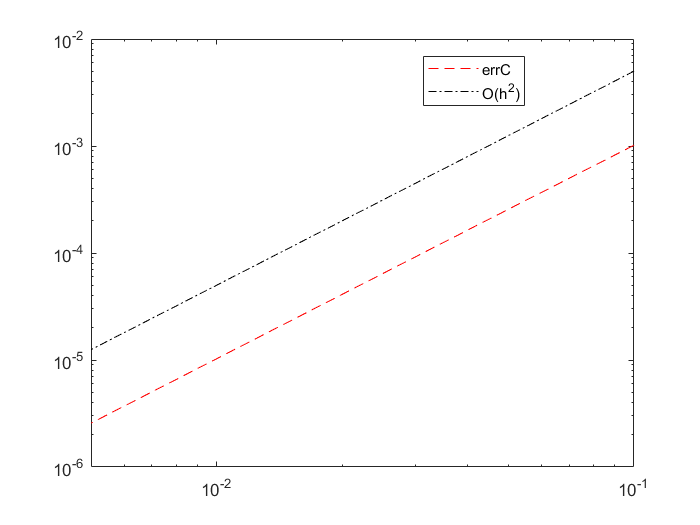
\includegraphics[scale=0.3]{中心差分和有限体积法的中矩形公式/errC.png}
\end{minipage}
}
\subfigure{
\begin{minipage}[t]{0.3\linewidth}
\centering
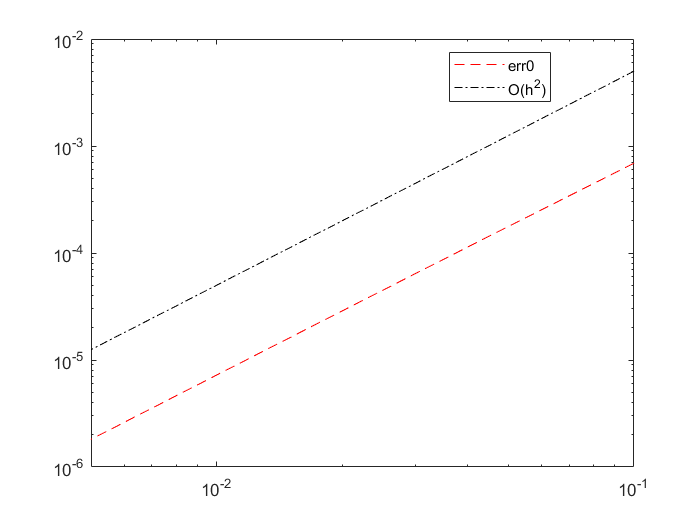
\includegraphics[scale=0.3]{中心差分和有限体积法的中矩形公式/err0.png}
\end{minipage}
}
\subfigure{
\begin{minipage}[t]{0.3\linewidth}
\centering
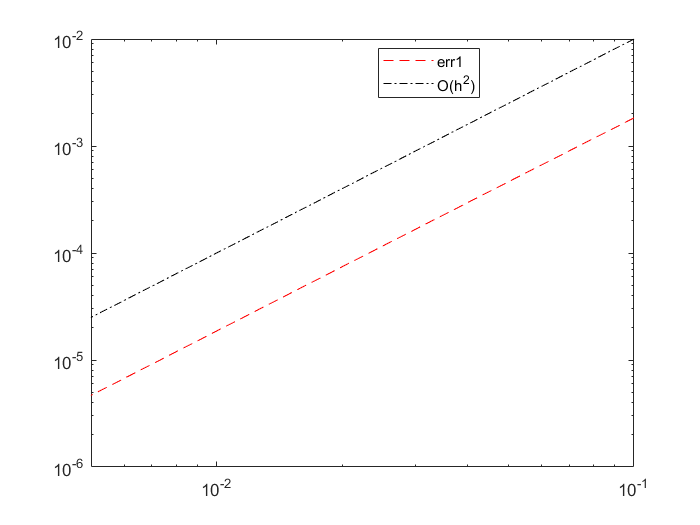
\includegraphics[scale=0.3]{中心差分和有限体积法的中矩形公式/err1.png}
\end{minipage}
}
\caption{\label{solution_image}误差估计图像}
\end{figure}

\begin{figure}[H]
\centering
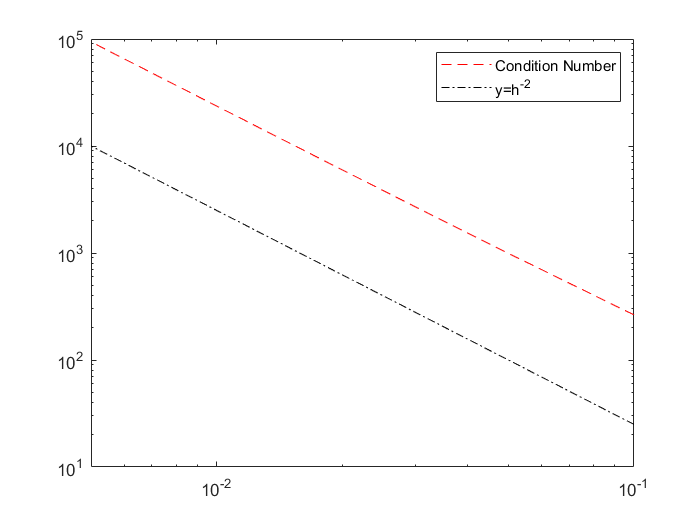
\includegraphics[scale=0.5]{中心差分和有限体积法的中矩形公式/CondA.png}
\caption{\label{CondA}$CondA$}
\end{figure}

\newpage
%-------------------------------------------------------------------
\subsection{中矩形公式}

下图是数值解和精确解的图像:
\begin{figure}[H]
\centering
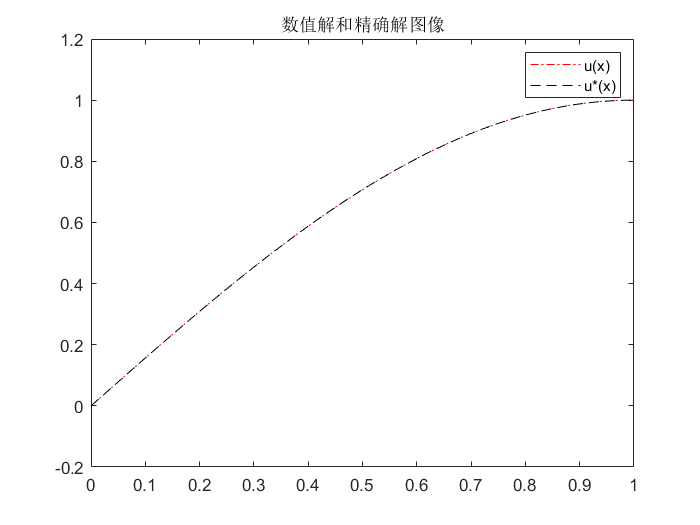
\includegraphics[scale=0.5]{中心差分和有限体积法的中矩形公式/solution_2.png}
\caption{\label{solution_image}数值解和精确解的图像}
\end{figure}

\begin{figure}[H]
\subfigure{
\begin{minipage}[t]{0.3\linewidth}
\centering
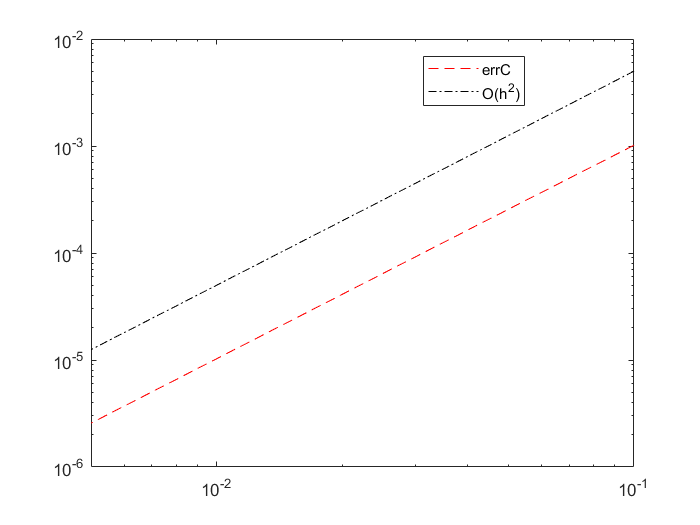
\includegraphics[scale=0.3]{中心差分和有限体积法的中矩形公式/errC.png}
\end{minipage}
}
\subfigure{
\begin{minipage}[t]{0.3\linewidth}
\centering
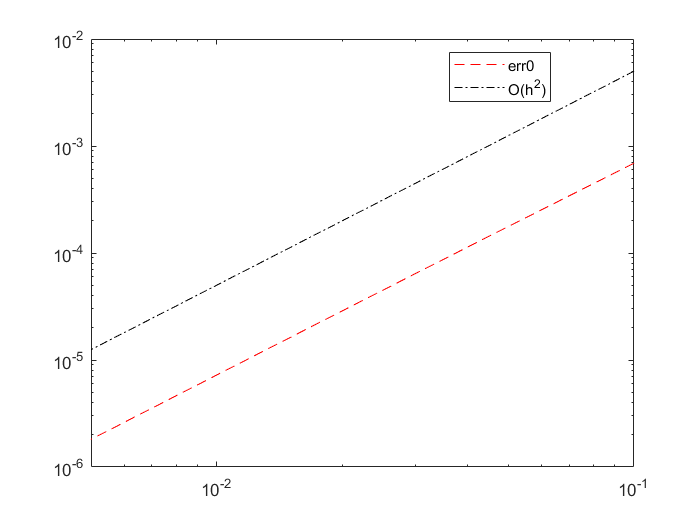
\includegraphics[scale=0.3]{中心差分和有限体积法的中矩形公式/err0.png}
\end{minipage}
}
\subfigure{
\begin{minipage}[t]{0.3\linewidth}
\centering
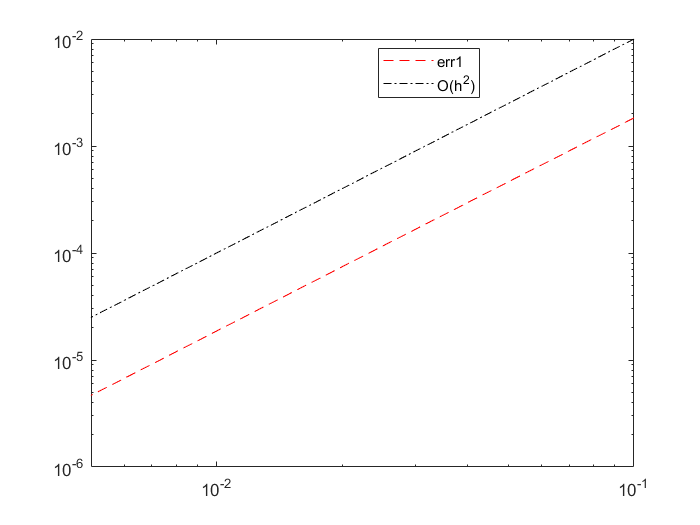
\includegraphics[scale=0.3]{中心差分和有限体积法的中矩形公式/err1.png}
\end{minipage}
}
\end{figure}

\begin{figure}[H]
\centering
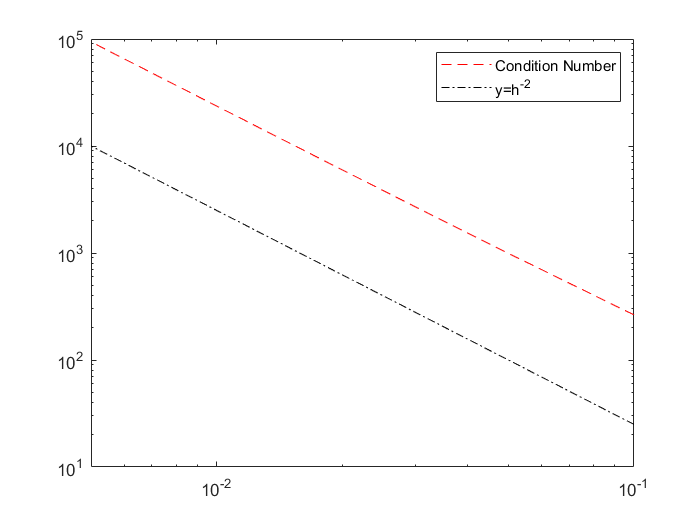
\includegraphics[scale=0.5]{中心差分和有限体积法的中矩形公式/CondA.png}
\caption{\label{CondA}$CondA$}
\end{figure}



%-----------------------------------------------------
\section{实验结果分析}
对于本题,向后差分法相应的三类类误差的收敛阶均为1,中心差分法和中矩形公式相应的三类误差均为2阶,矩阵A条件数有以下性质 $CondA$与同$h$成指数关系,且与$h^{-2}$同阶。
同一次有限元法做对比,errL的收敛阶从1变为2,收敛速度加快。

\end{document}